% Created 2018-04-15 Sun 03:41
% Intended LaTeX compiler: pdflatex
\documentclass[11pt]{report}
\usepackage[utf8]{inputenc}
\usepackage[T1]{fontenc}
\usepackage{graphicx}
\usepackage{grffile}
\usepackage{longtable}
\usepackage{wrapfig}
\usepackage{rotating}
\usepackage[normalem]{ulem}
\usepackage{amsmath}
\usepackage{textcomp}
\usepackage{amssymb}
\usepackage{capt-of}
\usepackage{hyperref}
\usepackage{minted}
\renewcommand\maketitle{}
\usepackage[margin=0.8in]{geometry}
\usepackage{amssymb,amsmath}
\usepackage{fancyhdr} %For headers and footers
\pagestyle{fancy} %For headers and footers
\fancyfoot[CE,CO]{}
\fancyhead[LE,LO]{}
\usepackage{lastpage} %For getting page x of y
\usepackage{float} %Allows the figures to be positioned and formatted nicely
\restylefloat{figure} %and this command
\usepackage{hyperref}
\hypersetup{urlcolor=blue}
\usepackage{titlesec}
\setcounter{secnumdepth}{4}
\usepackage{minted}
\setminted{frame=single,framesep=10pt}
\rfoot{\thepage\ of \pageref{LastPage}}
\usepackage[parfill]{parskip}
\usepackage{subfig}
\hypersetup{colorlinks=true,linkcolor=black, citecolor=black}
\usepackage{titlesec}
\usepackage{tabularx}
\usepackage{multicol}
\usepackage{array}
\newcolumntype{C}{ >{\centering\arraybackslash} m{11.4cm} }
\usepackage[usenames, dvipsnames]{color}
\usepackage[nocompress]{cite}
\renewcommand{\bibname}{References}
\usepackage{framed}
\usepackage{etoolbox}
\date{}
\title{\textbf{Modelling the effects of domestication in Wheat through novel computer vision techniques}}
\hypersetup{
 pdfauthor={Nathan Hughes},
 pdftitle={\textbf{Modelling the effects of domestication in Wheat through novel computer vision techniques}},
 pdfkeywords={},
 pdfsubject={},
 pdfcreator={Emacs 27.0.50 (Org mode 9.1.9)},
 pdflang={English}}
\begin{document}

\hyphenpenalty=10000

\titleformat{\chapter}[display]
   {\normalfont\huge\bfseries}{\chaptertitlename\ \thechapter}{20pt}{\Huge}
\titlespacing*{\chapter}{10pt}{10pt}{10pt}


% Redefine the plain page style
\fancypagestyle{plain}{%
  \fancyhf{}%
  \renewcommand{\headrulewidth}{0pt}% Line at the header invisible
  \rfoot{\thepage\ of \pageref{LastPage}}
  \fancyfoot[CE,CO]{}
}

% \patchcmd{\chapter}{\thispagestyle{fancy}}{\thispagestyle{fancy}}{}{}


\thispagestyle{empty}
\renewcommand{\headrulewidth}{0pt}
\begin{center}
  \fontsize{10}{12}
  \selectfont

  \textbf{\huge Modelling the effects of domestication in Wheat through novel computer vision techniques}

  \vspace{0.3in}

  \begin{tabular}[t]{ll}
    Author: & Mr. Nathan Hughes (nah26@aber.ac.uk) \\
    Supervisor: & Dr. Wayne Aubrey (waa2@aber.ac.uk) \\
    Degree Scheme &  G401 \hspace*{0.05in}(Computer Science)\\
    \\
    \\
    Date: & \today \\
    Revision: & 0.1\\
    Status: & Draft\\
    \\
  \end{tabular}
  \\
  \vspace{0.1in}
  This report was submitted as partial fulfilment \\of a BSc degree in Computer Science (G401)
\end{center}
\clearpage
\renewcommand{\headrulewidth}{1pt}

\thispagestyle{plain}

\begin{center}
  {\LARGE\bf Declaration of originality}
\end{center}

I confirm that:

\begin{itemize}
\item{This submission is my own work, except where
    clearly indicated.}

\item{I understand that there are severe penalties for Unacceptable Academic Practice, which can lead to loss of marks or even the withholding of a degree.}

\item{I have read the regulations on Unacceptable Academic Practice from the University's Academic Quality and Records Office (AQRO) and the relevant sections of the current Student Handbook of the Department of Computer Science.}

\item{In submitting this work I understand and agree to abide by the University's regulations governing these issues.}
\end{itemize}

\vspace{2em}
Name ............................................................  \\

\vspace{1em}
Date ............................................................ \\

\vspace{1em}
\begin{center}
  {\LARGE\bf Consent to share this work}
\end{center}

By including my name below, I hereby agree to this dissertation being made available to other students and academic staff of the Aberystwyth Computer Science Department.

\vspace{2em}
Name ............................................................  \\

\vspace{1em}
Date ............................................................ \\

\clearpage
\tableofcontents
\listoftables
\listoffigures
\listoflistings
\clearpage


\chapter{Introduction, Analysis and Objectives}
\label{sec:org3f5163d}

This project aims to answer a biological research question through the use of computer science, whilst also creating a software suite which will enable further studies to be carried out with ease.

Primarily the focus has been on the data science elements of my degree, creating, cleaning and discerning meaning in it.

Using a population of genetically diverse wheat, several hypothesis and questions are explored in the hopes of contributing to the scientific understanding of domestication. A mixture of image analysis through three-dimensional micro-computed tomography and computational analysis are used to provide these much needed solutions.

Additionally, as this is very much multi-disciplinary research, specific terms and definitions have been outlined in the \emph{glossary} (table:\ref{tab:orgcf3c942}).

\section{Background}
\label{sec:orge247ca5}

Western society and agriculture has been dominated by the ability to create successful crops for the past 10,000 years \cite{Ozkan2002}. Of these crops wheat is considered to be one of the most vital and is estimated to contribute to 20\% of the total calories and proteins consumed worldwide, and accounts for roughly 53\% of total harvested area (in China and Central Asia) \cite{Shiferaw2013}.

During domestication, the main traits selected for breeding were most likely plant height and yield. This meant that important non-expressed traits such as disease resistance and drought tolerance were often neglected and lost overtime.

Whilst the choices made for selective breeding were successful, effects are now being felt as it is estimated that as much as a 5\% dip is observed yearly on wheat production \cite{Shiferaw2013}. This decrease in efficiency is attributed to climate change bringing in more hostile conditions, which these elite and  domesticated genotypes are unprepared for.

Furthermore, with increasing populations and less arable land there is an even greater pressure for the optimisation of grain and spike characteristics. With studies showing that spikelet count can be controlled by specific and sometimes recessive genes \cite{Finnegan2018}, which could drastically enhance overall yield, and a general public distrust towards genetically modification \cite{Aleksejeva2014,Twardowski2015,Lynas} the reliance on breeding programs for optimisation is further stressed.

Modern breeding programs have had some success in selecting primitive undomesticated genotypes and using them to breed back in useful alleles which would have been lost during domestication \cite{Charmet2011}.

As such, there are questions still left open about how best to make selections for crop breeding. There is also a lack of formalised modelling of information which could be of use to these areas of research.

\section{Biological Question and Materials}
\label{sec:org9791efc}

The driving question for this research asks "Can \textmu{}-CT data be used to model domestication in wheat?". Using an already grown and harvested range of genetically diverse wheat this project has generated a collection of 3D images, processed these images into raw phenotypic data and produced biologically significant information.

The genotypes used in this study are listed here, denoted by "\emph{X} N" where \emph{X} indicates the ploidy. 2N - Diploid; 4N - Tetraploid; 6N - Hexiploid.

\begin{multicols}{3}

  \begin{itemize}
  \item Wild Monococcum (2N)
  \item Domesticated Monococcum (2N)
  \item Tauschii (2N)
  \end{itemize}

  \columnbreak

  \begin{itemize}
  \item Durum (4N)
  \item Dicoccoides (4N)
  \item Dicoccum (4N)
  \item Ispahanicum (4N)
  \item Timopheevii (4N)
  \end{itemize}

  \columnbreak

  \begin{itemize}
  \item Spelta(6N)
  \item Aestivum (6N)
  \item Compactum (6N)
  \end{itemize}

\end{multicols}
Full species names are found in table:\ref{tab:orgae2a748}.

\subsection{Why use \textmu{}-CT image analysis?}
\label{sec:orgef71fd3}
In the past, science has been greatly limited by the amount of data which could be processed in an experiment. In the last few decades the inclusion of computer science has reduced this bottleneck. Now, the challenge for many fields of research is producing more data and this is often cited as the major bottleneck in creating robust studies \cite{Furbank2011}.

Many experiments aim to meet the demand for data by using high-throughput automated imaging systems \cite{Naumann2007,Prasanna2013,Humplik2015}. These systems have, in the last decade, become a standard and accepted tool for data generation. However, they will only produce 2-dimensional data on a per-plant basis. Image processing research has had success in modifying these automated systems in order to produce a pseudo 3-dimensional structure using stero-imaging \cite{Roussel2016}. Even so, these techniques require destructive harvesting of materials and do not provide information of internal structure.

For decades medical research has found success with X-Ray imaging technology \cite{Wang2008}. From this, plant science has been able to benefit from the wealth of prior knowledge and more and more studies are being augmented with the use of X-Ray/\textmu{}-CT imaging \cite{Jhala2015,Tracy2012,Metzner2015,Hughes2017,Staedler2013}.

In this study, \textmu{}-CT has enabled the study of individual seeds of wheat, which is the product that plant breeders, commercial growers and farmers are truly interested in. Other imaging techniques could not provide as much detail, or in such a high throughput or quality.

\subsection{Extracted Data}
\label{sec:org2eee682}

These samples come from over 70 plants and provided in excess of 2000 seeds for analysis which data was created based on. The traits recorded are labelled in figure:\ref{fig:org5082162} and are as follows:

\begin{multicols}{2}

  \begin{itemize}
  \item Length
  \item Width
  \item Depth

  \end{itemize}

  \columnbreak

  \begin{itemize}
  \item Volume
  \item Surface Area
  \item Crease Depth / Volume
  \end{itemize}
\end{multicols}


\begin{figure}[htbp]
\centering
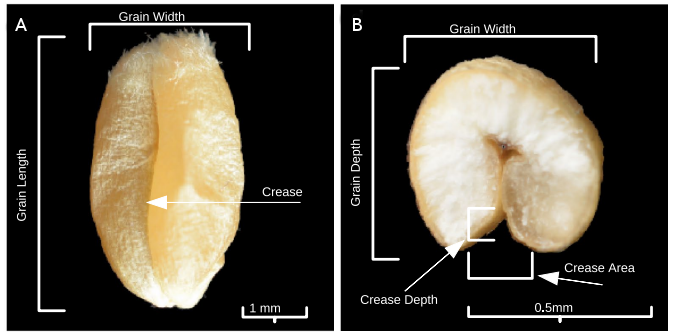
\includegraphics[width=17cm]{./images/seeds.png}
\caption{\label{fig:org5082162}
Wheat grain labelled (\emph{left}), wheat grain cut in half (\emph{right}), adapted from Hughes et al. \cite{Hughes2017}}
\end{figure}


\section{Significance to Current Research}
\label{sec:org6882cf3}
The biological interest in this area has been expressed in several areas of research \cite{Leigh2013}, it is proposed that the key to unlocking diversity in the wheat genus lies in these ancestor, undomesticated species \cite{Cockram2007}.

This research has the potential to be useful in several areas including: crop breeding; disease resistance; environmental stress. Each of these areas depend on making informed decisions in order to direct experiments. By producing information at an individual seed level, this study has been able to provide data that can offer suggestions of plant potential and behaviour.

Often, the most sought after traits are centred around thousand-grain-weight (TGW) as well as standard deviation of seed shapes. During harvesting, filters are used to only allow ideal shaped seeds through. This means that, potentially, despite a breed of wheat providing a high average volume of seed in reality much of it may go to waste if the shapes are not uniform. This research aims to alleviate this problem and provides low level information which is sorely required.

The individual images in figure:\ref{fig:org76b1c2a} show, at a glance, the diversity and also the difference in the wild and cultivated (domesticated)
species. This work allows for these differences to be quantified and evaluated into useful metrics for answering research based questions.

By better understanding the morphometric deviations in wheat species, more informed choices can be made when it comes to breeding wheat for the future and to fulfil ever-changing requirements.

\clearpage

\begin{figure}[htbp]
\centering
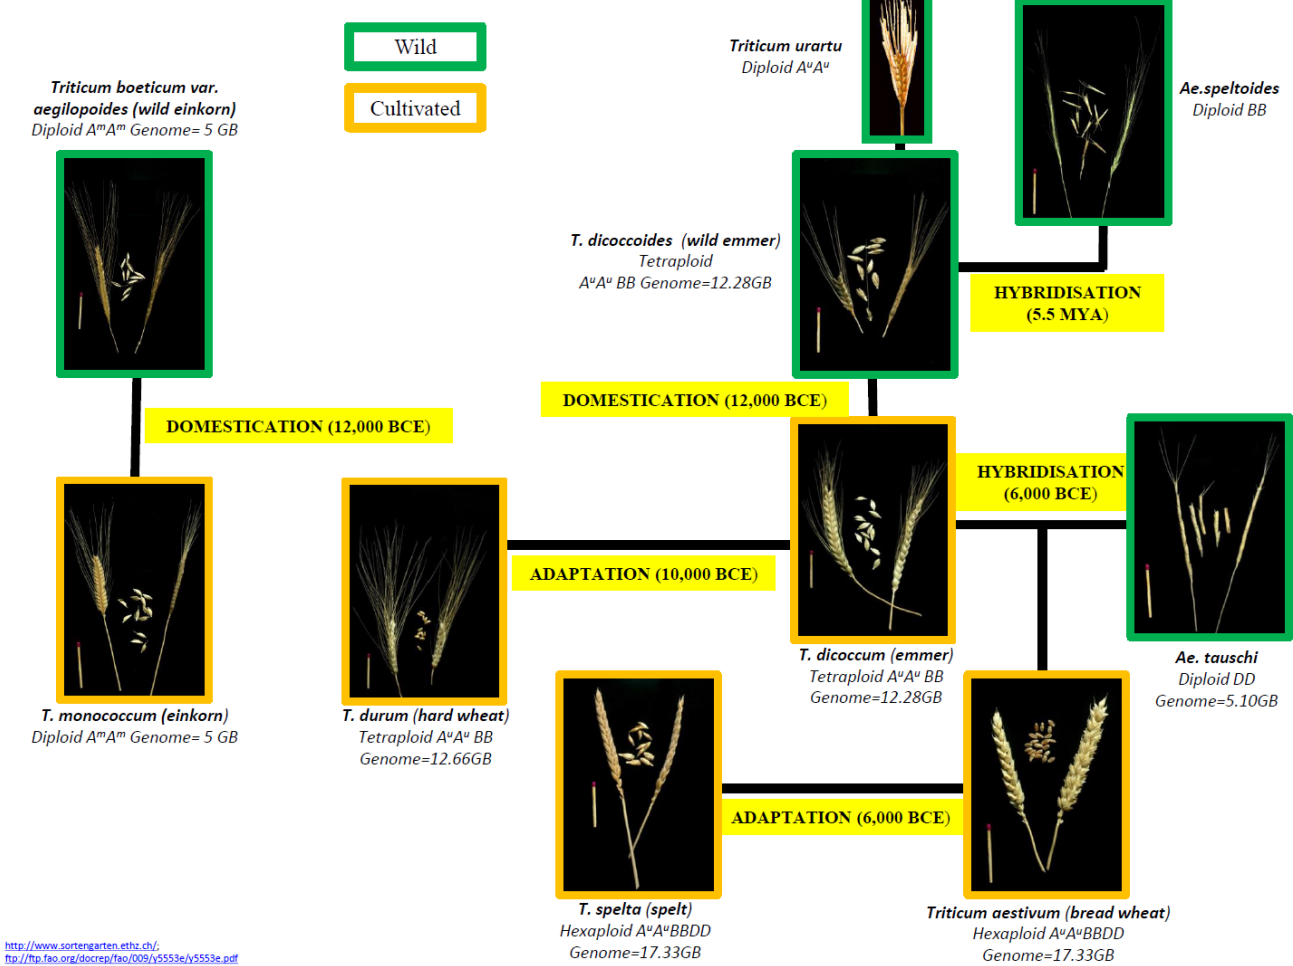
\includegraphics[width=17cm]{./images/philotree.png}
\caption{\label{fig:org76b1c2a}
Phylogeny of wheat genotypes (Provided by Dr. Hugo Oliveira)}
\end{figure}

\section{Aims and Objectives}
\label{sec:orge7425c1}

The overarching aim of this project has been to create several pieces of software which aid in answering the biologically significant questions outlined. As well as to prove/disprove the hypothesis stated below.

The software created is robust in order to duplicate results and is flexible as to allow for further studies to be carried out and to use the same method.

Novel additions have been made to existing image analysis libraries in order to make them more flexible for this project. Figure:\ref{fig:org5b5d308} illustrates the range of diversity

Furthermore, the library written allows for easy data organisation and automation of otherwise difficult tasks such as concatenating data from multiple sources and graphing of information. Full documentation and integrated testing allows for a suite of tools which can be built upon in future and reduce the amount of effort required for similar studies to be carried out and analysed.

These aims have a focus on the phenotypic attributes generated from customised image analysis software \cite{Hughes2017} and can be seen in figure:\ref{fig:org5082162}.


\section{Hypothesis}
\label{sec:orge9705a6}
To provide a full spectrum of analysis the null-hypothesis of this work is presented as investigating if there are morphometric differences in the seeds of several wheat varieties outlined in figure:\ref{fig:org76b1c2a}.

The comparison pairs are as follows:

\begin{enumerate}
\item Monococcum Wild and Monococcum Domesticate
\item Dicoccoides and Dicoccum
\item Spelta and Aestivum
\item Dicoccum and Durum
\item Monococcum Wild and Dicoccoides
\end{enumerate}


\begin{figure}[htbp]
\centering
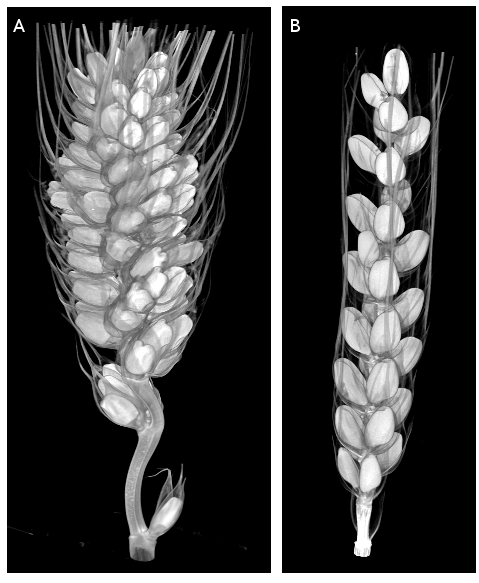
\includegraphics[width=10cm]{./images/spikes.png}
\caption{\label{fig:org5b5d308}
Scans of wheat, showing diversity in Population, Compactum (6N) left, Durum right (4N)}
\end{figure}

\section{Challenges Overview}
\label{sec:org734b86c}

The challenges which this project tackles come in two flavours: Computational and Biological. As such keen awareness of these is needed to appreciate the novelty of this work.

\subsection{Biological Challenges}
\label{sec:orga0ce7e6}
Previous studies have been able to demonstrate that variation in wheat grain morphology can be partially explained, in 2010 Gegas et al. demonstrated this through a 99.4\% 2 component PCA \cite{Gegas2010}. However there is much left to do in terms of formal classifications and descriptions of these differences. This project deals with this problem through computational analysis.

Two effects run parallel in this study which requires acute biological knowledge of in order to make correct decisions:

\begin{enumerate}
\item The effects of ploidy in wheat.
\item The effects of domestication in wheat.
\end{enumerate}

Hypothesis are required to take into account, both of these effects so as not to misidentify results.

\subsection{Computational Challenges}
\label{sec:org10dbbca}
Using \textmu{}-CT data in plant sciences is becoming more and more common \cite{Tracy2017,Jhala2015,Hughes2017,Metzner2015} and whilst a lot of studies focus on the traits of grains specifically no formal model has been created, no accepted data format. This is a data engineering problem and the methods described in this project address this.

Further to data organisation, proposals are made for the statistical analysis which should be used. This allows for studies to become more robust and repeatable, thus strengthening the studies overall.

The biological material used in this research is much more diverse a population than has been previously studied with \textmu{}-CT image analysis, this requires current computer vision methods to be adapted in order to be accurate.

\section{Deliverables}
\label{sec:org7e67c86}

This project provides three final deliveribles:

\begin{enumerate}
\item A flexible software suite written in \emph{Python} that provides a standardised method for analysing and interpreting \textmu{}-CT data output.
\item A Graphical User Interface (GUI) which offers a point and click method for data gathering, graphing and manipulating \textmu{}-CT data, using the library from deliverable 1 as a backend.
\item Answers to the proposed questions (hypothesis), the \emph{Results} and \emph{Discussion} sections of this report provides this.
\end{enumerate}

\chapter{Software Design, Implementation and Testing}
\label{sec:org2ebc689}
This chapter outlines choices and methodologies employed in the software engineering aspect of this project, as well as highlighting the key functional requirements and implementation decisions.

\section{Functional Requirements}
\label{sec:org9415b99}
Requirements for this project are split between software requirements for both the CT Analysing Library and the CT GUI Application and the research requirements (i.e. the answers to the proposed hypothesis). Here the requirements for the software are discussed:
\subsection{Requirements for CT Analysing Library}
\label{sec:org1bf5993}

These are the functional requirements for the Python library produced:

\begin{multicols}{2}

  \begin{itemize}
  \item Provide an OOP means to deal with data
  \item Make gathering of data simplified
  \item Handle Saving of data in a useable format
  \item Easily enable data transformations
  \item Perform hypothesis testing
  \end{itemize}

  \columnbreak

  \begin{itemize}
  \item Process rejoining of split scans
  \item Handle Removing of erroneous data
  \item Enable matching data to external information
  \item Auto plot data (boxplots, histograms etc.)
  \item Allow easy filtering of data
  \end{itemize}

  \columnbreak

\end{multicols}

\subsection{Requirements for CT GUI Application}
\label{sec:orgf4481d3}

\begin{multicols}{2}

  \begin{itemize}
  \item Provide a intuitive user interface for working with CT data
  \item Allow a interaction with data without the need for programming
  \item Implement the Matplotlib plotting utility
  \item Easily join experiment data with CT data
  \item Use an MVC model
  \end{itemize}

  \columnbreak

  \begin{itemize}
  \item Implement the CT Analysis Library
  \item Display data visually
  \item Dynamically create graphs
  \item Provide hypothesis testing
  \end{itemize}

  \columnbreak

\end{multicols}

\section{Software Development Methodology}
\label{sec:org387a191}
This project made use of formal design methods and strict organisation whilst being flexible to change. Overall the design took a hybridised form in order to best suit the scientific environment which this domain specific software is built for.

Data analysis drove the direction of the project, as a result an agile methodology was adopted.
Weekly sprints were implemented as a list of "todo's", these were written on a Monday morning based off of the previous week's list.

Critical self-evaluation was performed by means of a "one-man SCRUM" meeting, this is a technique which requires self-discipline in order to accurately find faults and areas for improvement \cite{Andrews}.

Further to this, regular meetings with research staff, at the National Plant Phenomics Centre,  allowed for a developer-client relationship which SCRUM defines as being key. During these meetings details of the research was discussed and ideas given as to how future experiments could proceed. This allowed for critical decisions to be made as to software design and overall structure.
\section{Language Choices}
\label{sec:org06dbf74}
Both the CT Analysing Library and the CT Analysing GUI are implemented using the Python programming language, it has been developed and tested in versions 3.5 and 3.6 (Python 2 is not supported at all by this project).

In scientific programming three of the most commonly used languages are Python, R and MATLAB \cite{Ozgur2016}.

These three languages are able to provide all the features which this project requires. However Python was chosen for several reasons.

MATLAB could not be used as a potential language due to it being pay to use software, as this project aims to be accessible, the cost of software would greatly reduce the scope of access.

R is a valid candidate, it provides all of the statistical capabilities required by the project, it also provides packages for creating GUI based applications, it is fast and it is widely used in scientific computing and data science.

The main deciding factor is Python's wealth of resources, adoption rate and the developer of this project being vastly more experienced with Python's ecosystem than R's.

\section{Designing Process}
\label{sec:org0b49482}
Through meetings and emails, the agile principles of communication over comprehensive documentation was used. Where conversations were decidedly much more beneficial than complex planing prior to developing a product.

Graphical elements, such as the graphing functionality of the CT Analysing Library and the CT GUI Application were sketched using wire-frames whilst in meetings where the potential users (clients) could provide their ideas.

In figure:\ref{fig:orgde08609} an example of the wire-frames created during meetings is show (A), next to it is displayed the final look of the loading window (B).
\begin{figure}[htbp]
\centering
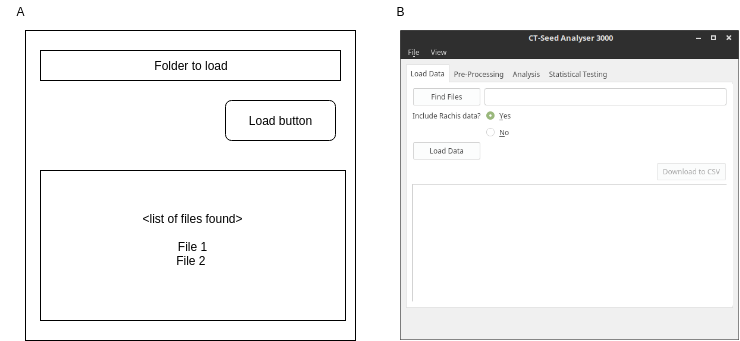
\includegraphics[width=16cm]{./images/wireframe1.png}
\caption{\label{fig:orgde08609}
Wire-frame of the GUI loading data window}
\end{figure}

Similarly, figure:\ref{fig:org66ff531} provides the initial wire-frame (A) of how the analysis window could have looked and what kind of GUI elements would be required, again, next to it is the final analysis window (B)
\begin{figure}[htbp]
\centering
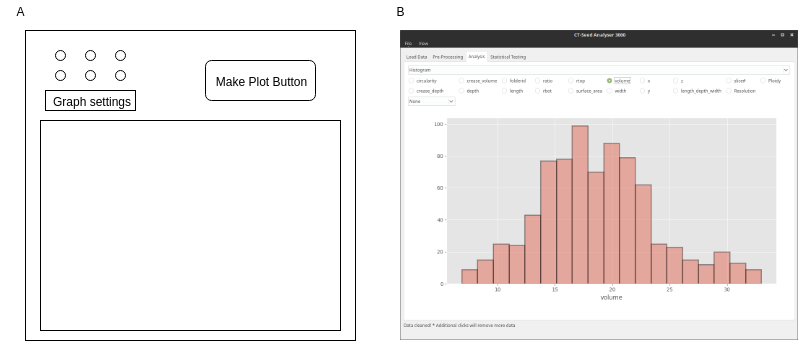
\includegraphics[width=16cm]{./images/wireframe2.png}
\caption{\label{fig:org66ff531}
Wire-frame of the GUI analysis window}
\end{figure}
\section{Documentation}
\label{sec:org8ec98c8}
Whilst an agile approach was used, some documentation was created for use with the CT Analysing Library.

The provided CT Analysing Library comes with "human-readable" format. Where most documentation generators (Doxygen, Pydocs, Javadocs etc.) implement very well structured and comprehensive documentation, the output is generally not very friendly and easy to read. Particularly for non-career-programmers. A core feature of these provided software implementations are that they are well suited for a biologist, researcher or statistician to use.

This documentation generator was purpose created, implemented in LISP and provided in listing:\ref{orgdbf3e7b}.

Beyond this, inline commenting is provided for supplied software. Keeping in line with the agile development ethos the software is self-documented and self-evident. A brief example of this is shown in listing:\ref{org9305c03}

Documentation for the CT GUI application is provided as a visual user guide, and provides sample data for the user to test with.
\section{Software Library Choices}
\label{sec:orgc2e311b}
The software libraries used for this project focus around data manipulation, where possible core libraries of the Python language were used and only well supported, established and documented libraries were chosen. Software support is a major requirement for reproducible results.

All software packages used in the Analysing Library are required by the CT Analysing GUI as the Library is a dependency of it. The GUI has a single separate requirement \emph{PyQT5}.
Table:\ref{tab:orgd84b275} contains a full listing of all software used and required by this project.
\subsection{CT Analysing Library}
\label{sec:orgb8ae430}
\subsubsection{Numpy}
\label{sec:org40fd166}
The Numpy library is one of the most commonly used additions to the Python ecosystem, it is fundamental to many data science projects. Here it is used to handle data lists, arrays and structures. There is no viable alternative to this package and it is required by Scipy and Statsmodels.
\subsubsection{Matplotlib/Seaborn}
\label{sec:orgc9ab95b}
Matplotlib acts as the plotting backend for the project. The Seaborn package acts as a porcelain for matplotlib and makes graph creation and decoration much easier.
\subsubsection{Scipy}
\label{sec:orgf78f6d6}
Data transforms such as Box Cox and PCA are dependant on the functions of the Scipy library. Alternatives are available, however this is the most well established and often used library for these functions.
\subsubsection{Pandas}
\label{sec:orgb3a541c}
Pandas is used to read the CSV files which the raw data is stored in. This library converts and stores data in dataframes which are used throughout this project to manipulate data.
\subsubsection{Xlrd}
\label{sec:orgc26186d}
This extension library is required in order to read Microsoft encoded files. Extra experiment information can be provided with the "xlsx" extension.
\subsubsection{Statsmodels}
\label{sec:org0fc0d8a}
Bayesian hypothesis testing is provided through this library.
\subsubsection{PyQT5}
\label{sec:orgcfd2c5f}
There were many options for creating a user interface in Python, the language provides its own core library via the \emph{TKinter} module. However PyQT is a port of the QT framework, one of the most widely used libraries for GUIs in software development. It is cross platform, robust and has excellent documentation and user-guides.

\section{Implementation}
\label{sec:org1078b59}
Strict software engineering principles were applied during creation of this project. The use of standards, design patterns and code-linters have been used throughout to minimise the possibility of errors and to create wholly extendable software. These devices enable understandable and self-documented code allowing future users to quickly start using the provided packages.

\subsection{Design Patterns}
\label{sec:orgfcd65d6}
Each of the packages of this projects follow a design pattern to make them extendable for future additions, as and when they are required by future studies and experiments.
\subsubsection{CT Analysing Library Design Pattern}
\label{sec:org1d194b4}
The CT Analysing Library uses a Singleton style design pattern. A single data object is created from a \emph{CTData} class.

A very functional paradigm is used by this library. By applying mapping and filter style functions data elements can be passed to the supporting modules: \emph{data\_transforms.py}; \emph{graphing.py}, \emph{statistical\_tests.py}. These modules enable scientific functions to be applied to the \emph{CTData} object. A UML style class diagram is shown in figure:\ref{fig:orge392a34}, here the interactions of the classes can be seen, as well as their internal functions.
\begin{figure}[htbp]
\centering
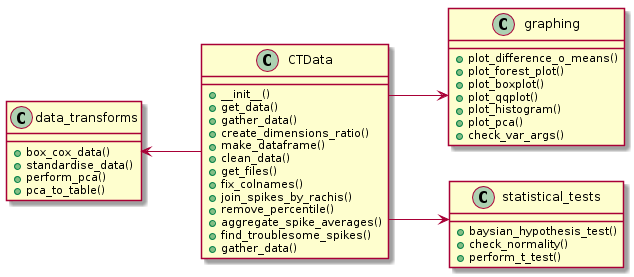
\includegraphics[width=12cm]{./images/ctdata.png}
\caption{\label{fig:orge392a34}
CT Analysing Library UML}
\end{figure}

\subsubsection{CT GUI Application Design Pattern}
\label{sec:org0c42171}
The Model-View-Controller (MVC) design pattern is one of the most commonly structures for creating user interfaces. It allows for the user's view/interface code to be separated from the model, the code which changes the data. The model and the view communicate and update each other via the controller element of the design. The QT framework provides "connectors" which act as triggers/activations for functions, these are set off by the user providing either keyboard or mouse based input.

\begin{figure}[htbp]
\centering
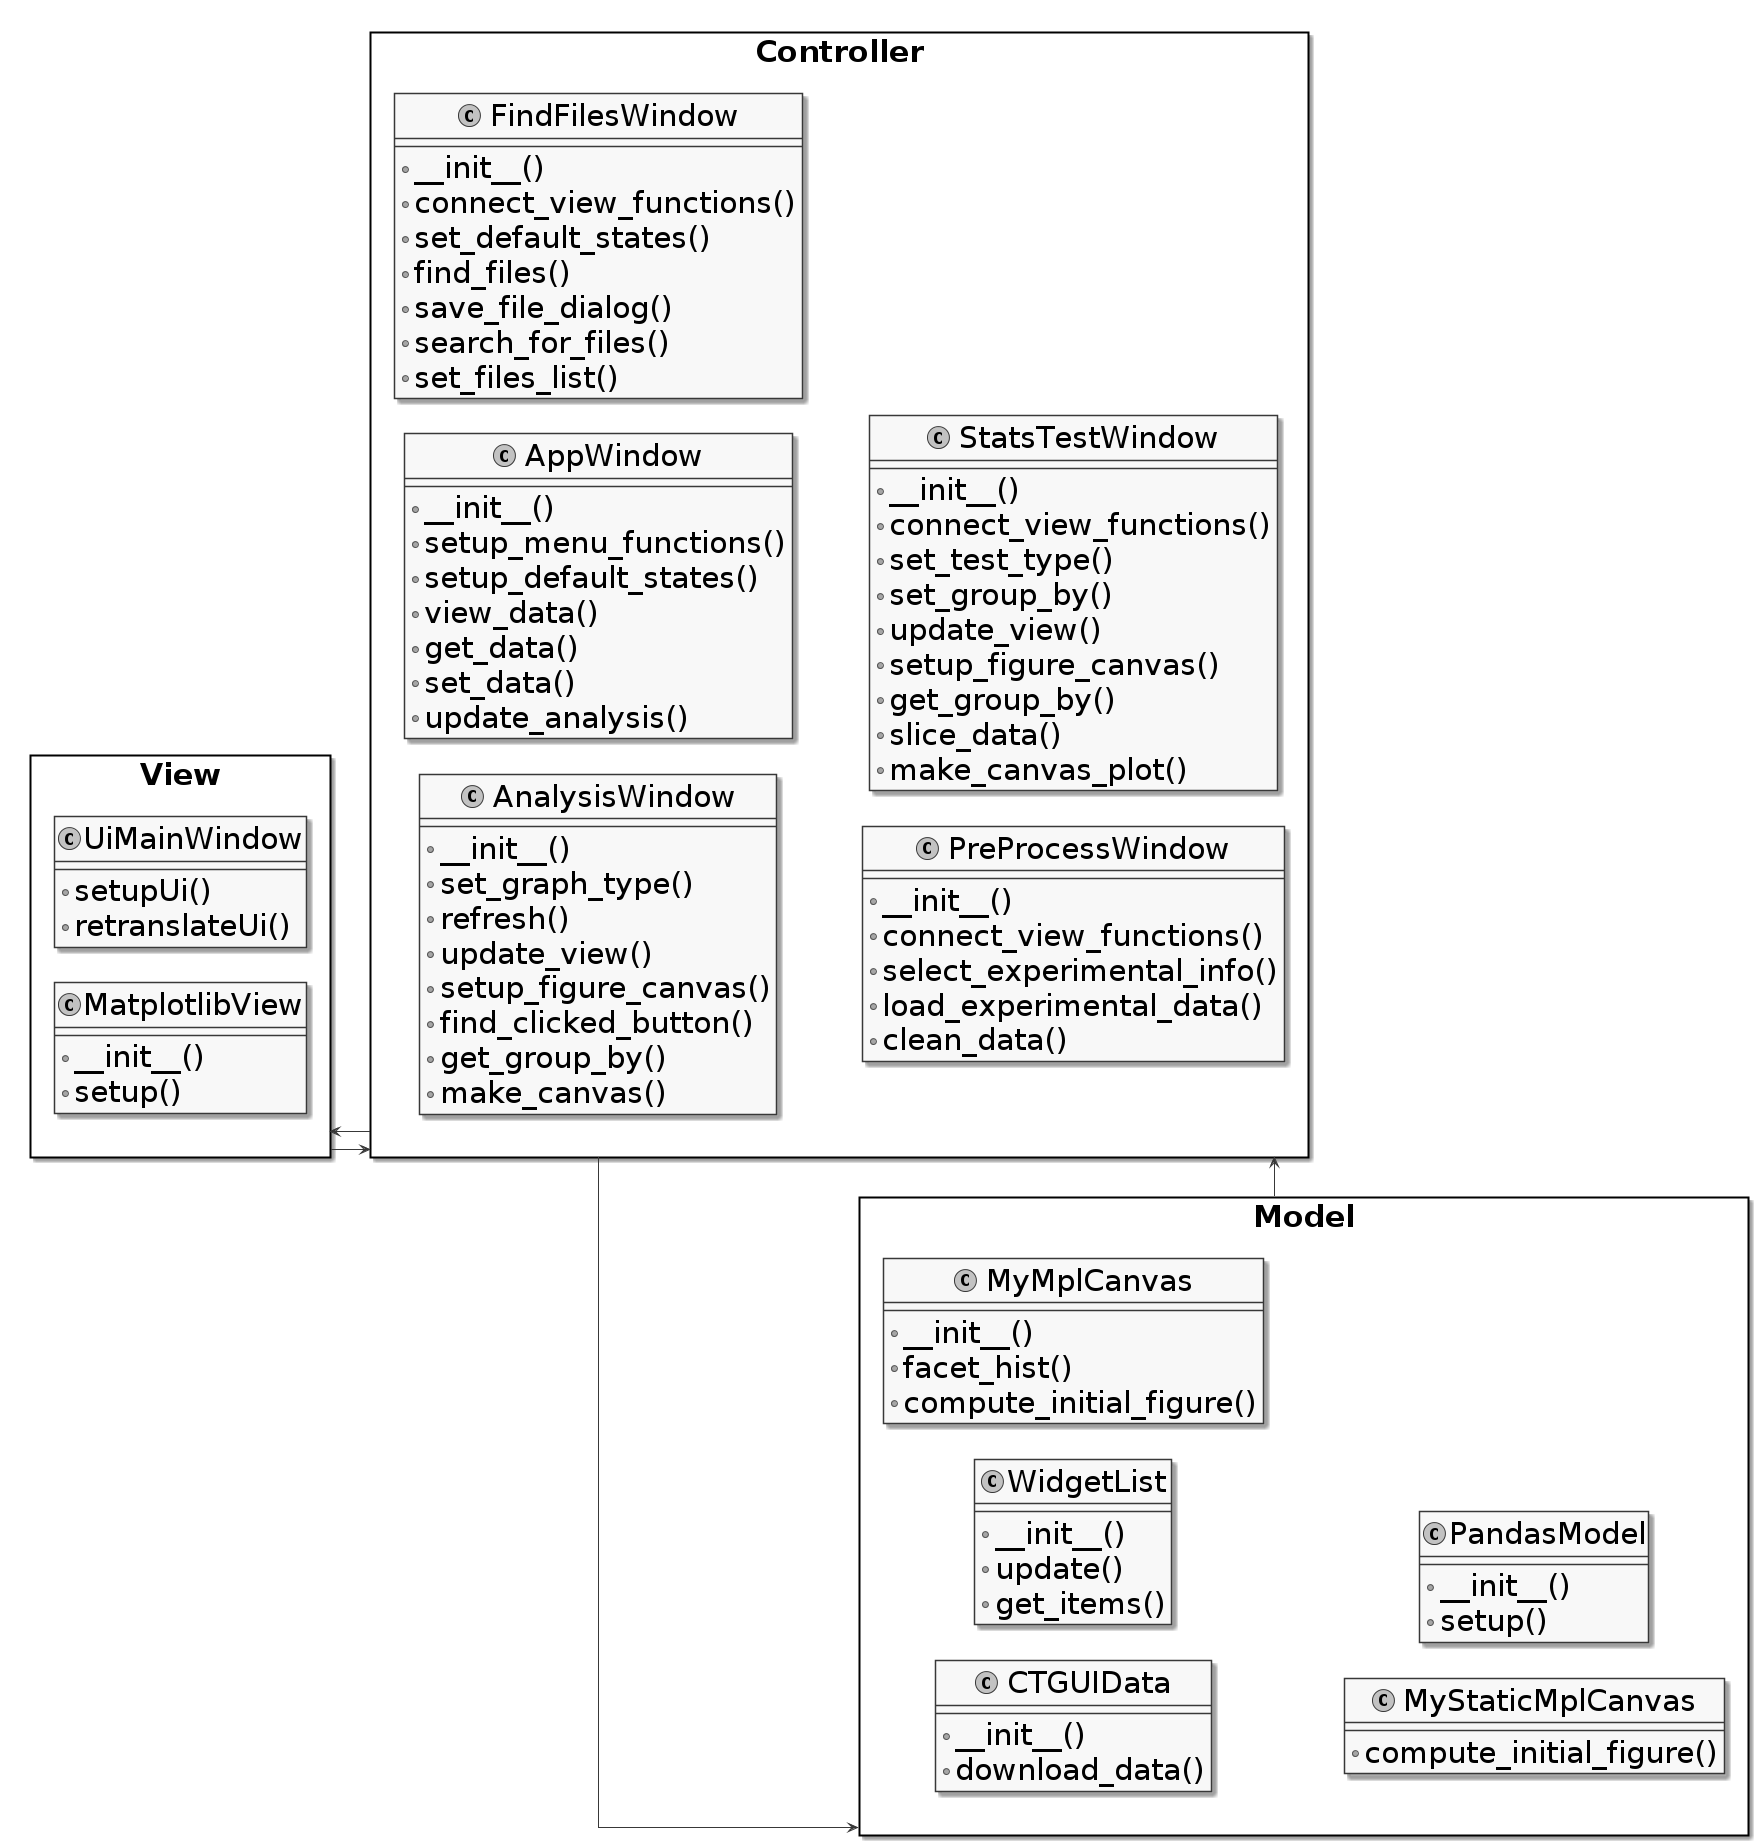
\includegraphics[width=15.2cm]{./images/ctgui.png}
\caption{\label{fig:orge783e20}
CT Analysing GUI UML}
\end{figure}


\subsection{Standards}
\label{sec:orge25cccc}
The main standard adhered to for software provided by this project is the PEP8 style guide \cite{VanRossum}. The principle behind this coding style, as stated by Guido van Rossum, is "Code is read much more often than it is written". This makes this styling guide perfect for the chosen agile methodology of self-evident documentation in the software.

In addition to PEP8, a Python code linter Flake8 has been used to prevent "code smells", bad formatting, incorrect white space usage etc.

\section{Version control}
\label{sec:org991df07}
This project has used Git version 2.7.4 throughout. The structure of the project has been as submodules of a larger project.

By using submodules the CT Grain Analysing Library could be kept in sync with the GUI aspect of the project.

Additionally, \emph{setup.py} has been used to provide installation of the library, the code for this can be seen in listing:\ref{orgd09a84d}.
\section{Testing}
\label{sec:org48b4e0e}
\subsection{Feedback Forms}
\label{sec:org902c110}
Feedback and constructive suggestions were made by researchers at the National Plant Phenomics Centre, these were submitted via the Google forms service\ldots{}
\subsection{Unit Testing CT Analysing Library}
\label{sec:org721f763}
TODO
\begin{table}[htbp]
\caption{\label{tab:org81bc5c0}
Output of \emph{pytest} Unit Tests and results for CT Analysing Library}
\centering
\begin{tabularx}{\textwidth}{|l|X|}
\hline
\textbf{Result} & \textbf{Test}\\
\hline
\color{ForestGreen}Passed & CTData.py::test\_aggregate\_spike\_averages\\
\hline
\color{ForestGreen}Passed & CTData.py::test\_clean\_data\_maximum\_removed\\
\hline
\color{ForestGreen}Passed & CTData.py::test\_clean\_data\_minimum\_removed\\
\hline
\color{ForestGreen}Passed & CTData.py::test\_load\_additional\_data\\
\hline
\color{ForestGreen}Passed & CTData.py::test\_load\_additional\_data\_no\_data\\
\hline
\color{ForestGreen}Passed & CTData.py::test\_load\_data\\
\hline
\color{ForestGreen}Passed & CTData.py::test\_NoDataFoundException\\
\hline
\color{ForestGreen}Passed & Data\_transforms.py::test\_box\_cox\_data\\
\hline
\color{ForestGreen}Passed & Data\_transforms.py::test\_pca\_to\_table\\
\hline
\color{ForestGreen}Passed & Data\_transforms.py::test\_perform\_pca\\
\hline
\color{ForestGreen}Passed & Data\_transforms.py::test\_standardise\_data\\
\hline
\color{ForestGreen}Passed & Graphing.py::test\_plot\_boxplot\_as\_dataframe\\
\hline
\color{ForestGreen}Passed & Graphing.py::test\_plot\_boxplot\_as\_object\\
\hline
\color{ForestGreen}Passed & Graphing.py::test\_plot\_difference\_of\_means\\
\hline
\color{ForestGreen}Passed & Graphing.py::test\_plot\_histogram\_as\_dataframe\\
\hline
\color{ForestGreen}Passed & Graphing.py::test\_plot\_histogram\_as\_object\\
\hline
\color{ForestGreen}Passed & Graphing.py::test\_plot\_pca\\
\hline
\color{ForestGreen}Passed & Graphing.py::test\_plot\_qqplot\\
\hline
\color{ForestGreen}Passed & Statistical\_tests.py::test\_baysian\_hypothesis\_test\\
\hline
\color{ForestGreen}Passed & Statistical\_tests.py::test\_t\_test\\
\hline
\color{ForestGreen}Passed & Statistical\_tests.py::test\_test\_normality\\
\hline
\end{tabularx}
\end{table}

\subsection{Unit Testing CT GUI Application}
\label{sec:org60177be}
TODO

\begin{longtable}{|l|p{4.4cm}|C|}
\caption{\label{tab:org80ab810}
Output of \emph{pytest} Unit Tests and results for CT GUI Application}
\\
\hline
\textbf{Result} & \textbf{Test} & \textbf{Image}\\
\hline
\endfirsthead
\multicolumn{3}{l}{Continued from previous page} \\
\hline

\textbf{Result} & \textbf{Test} & \textbf{Image} \\

\hline
\endhead
\hline\multicolumn{3}{r}{Continued on next page} \\
\endfoot
\endlastfoot
\hline
\color{ForestGreen}Passed & analysis.py:: box\_groupby\_1\_rb\_1 & \begin{center}
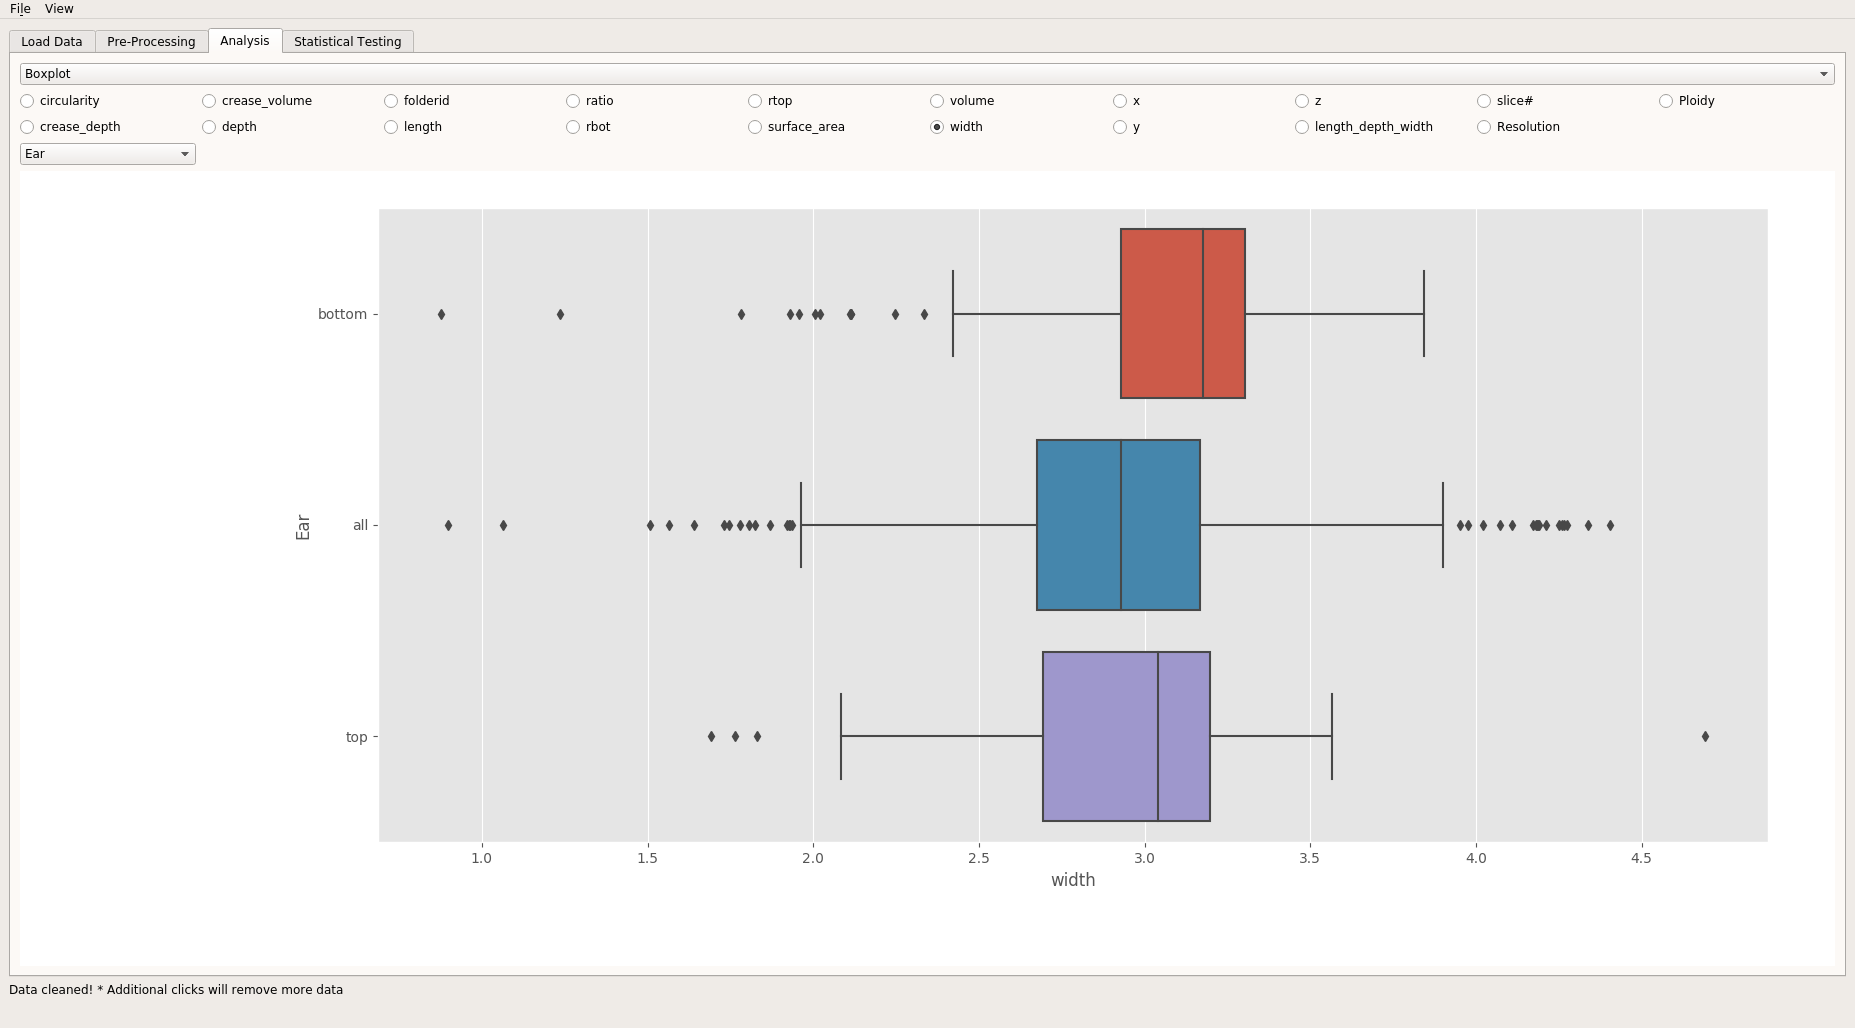
\includegraphics[width=.9\linewidth]{./images/Screenshots/analysis_window_box_groupby_1_rb_1.png}
\end{center}\\
\hline
\color{ForestGreen}Passed & analysis.py:: box\_groupby\_2\_rb\_2 & \begin{center}
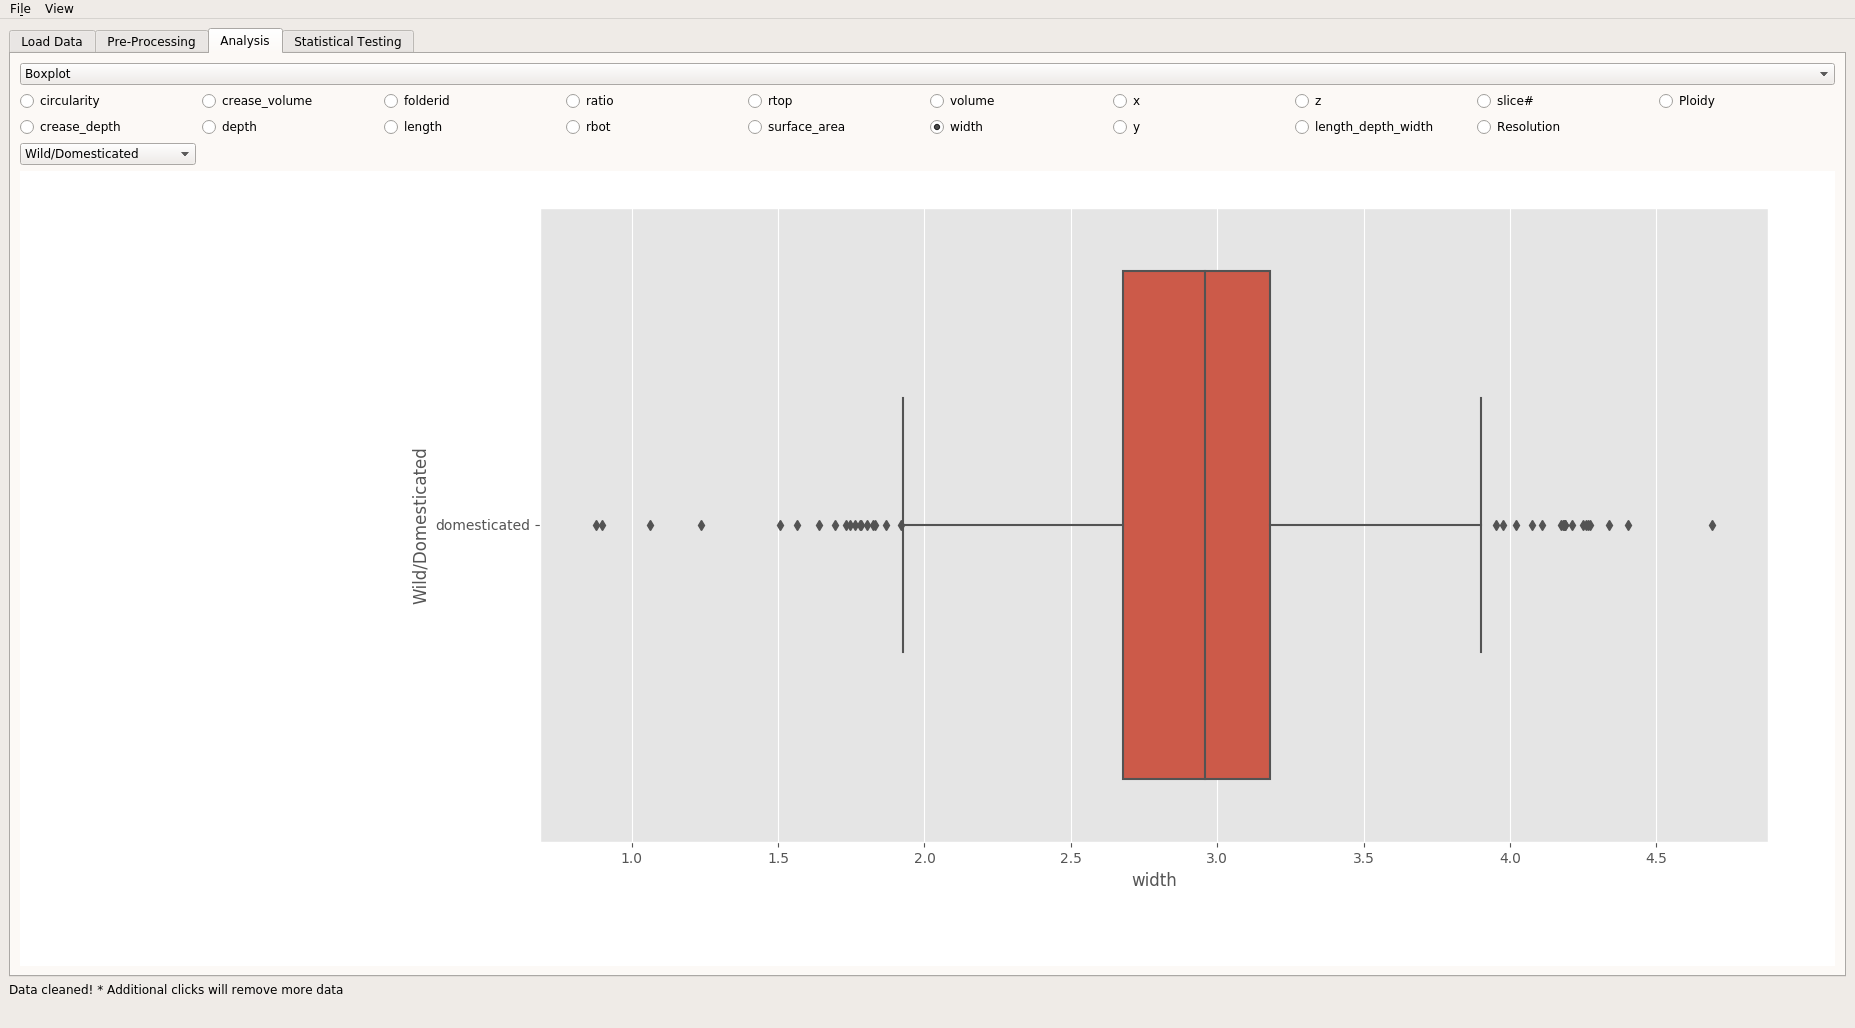
\includegraphics[width=.9\linewidth]{./images/Screenshots/analysis_window_box_groupby_2_rb_2.png}
\end{center}\\
\hline
\color{ForestGreen}Passed & analysis.py:: box\_rb\_1 & \begin{center}
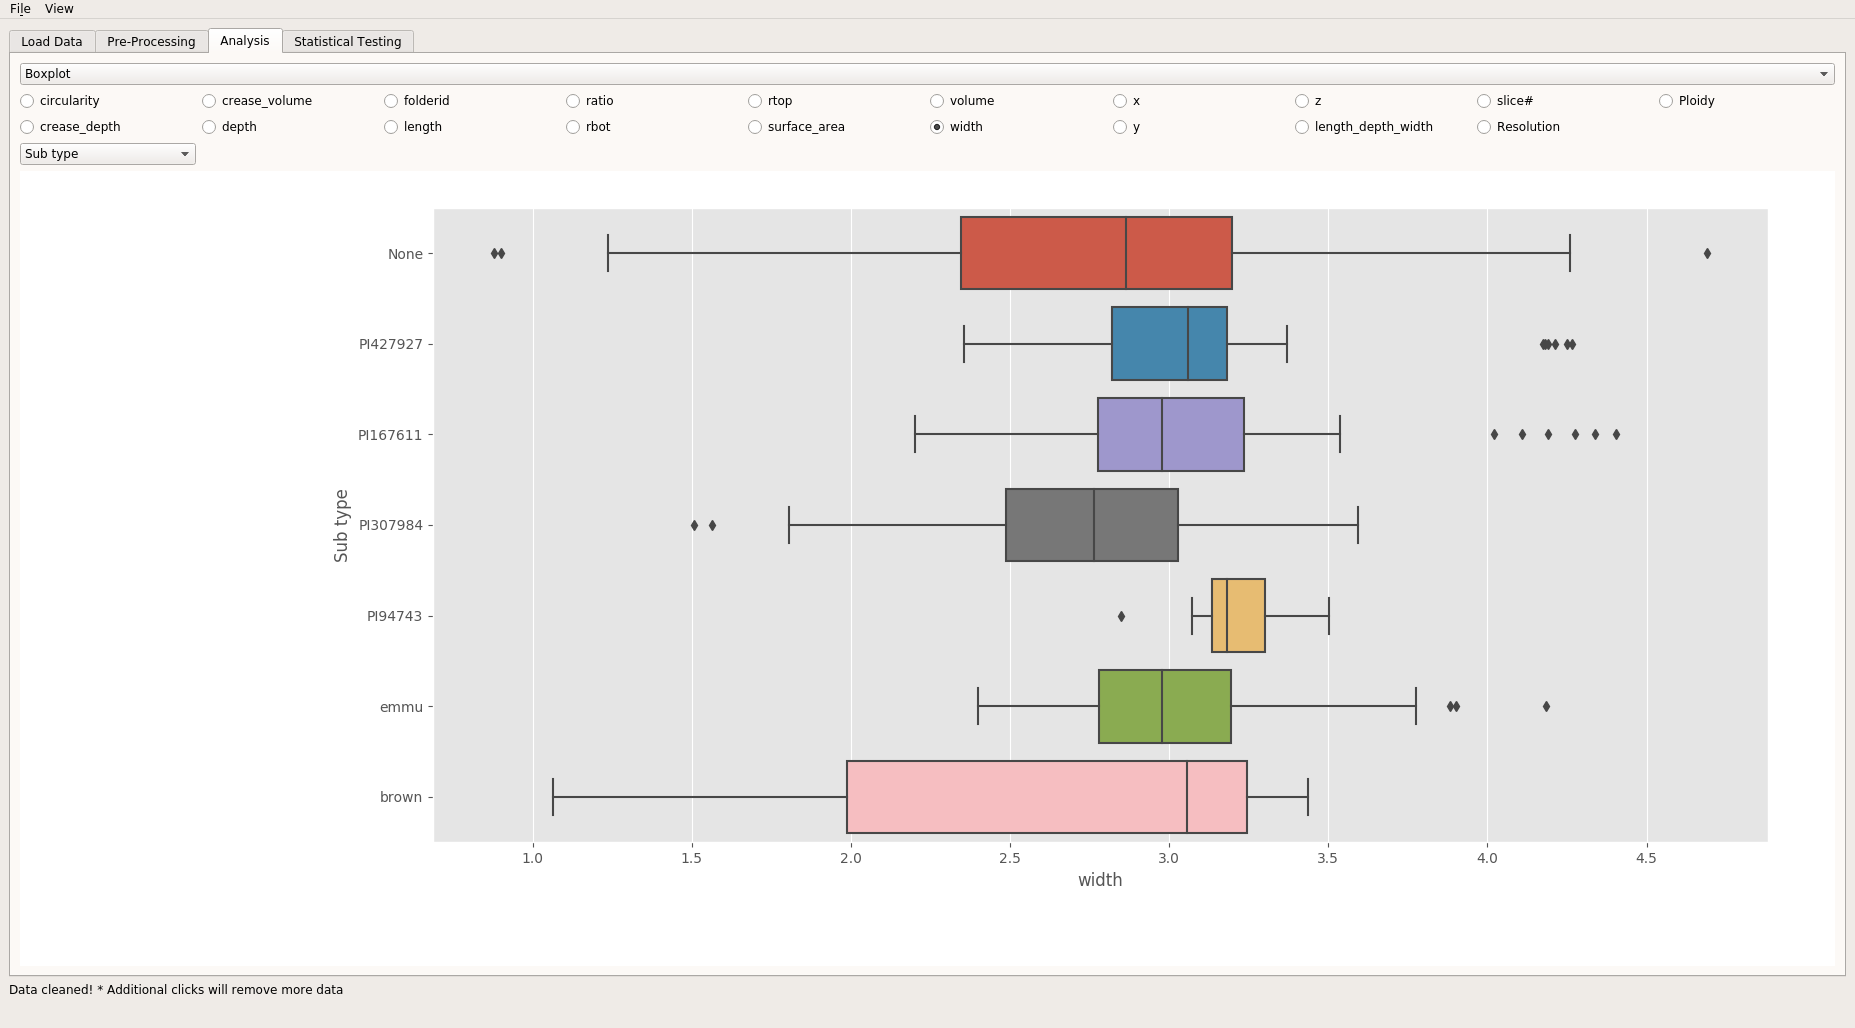
\includegraphics[width=.9\linewidth]{./images/Screenshots/analysis_window_box_rb_1.png}
\end{center}\\
\hline
\color{ForestGreen}Passed & analysis.py:: hist\_groupby\_1\_rb\_1 & \begin{center}
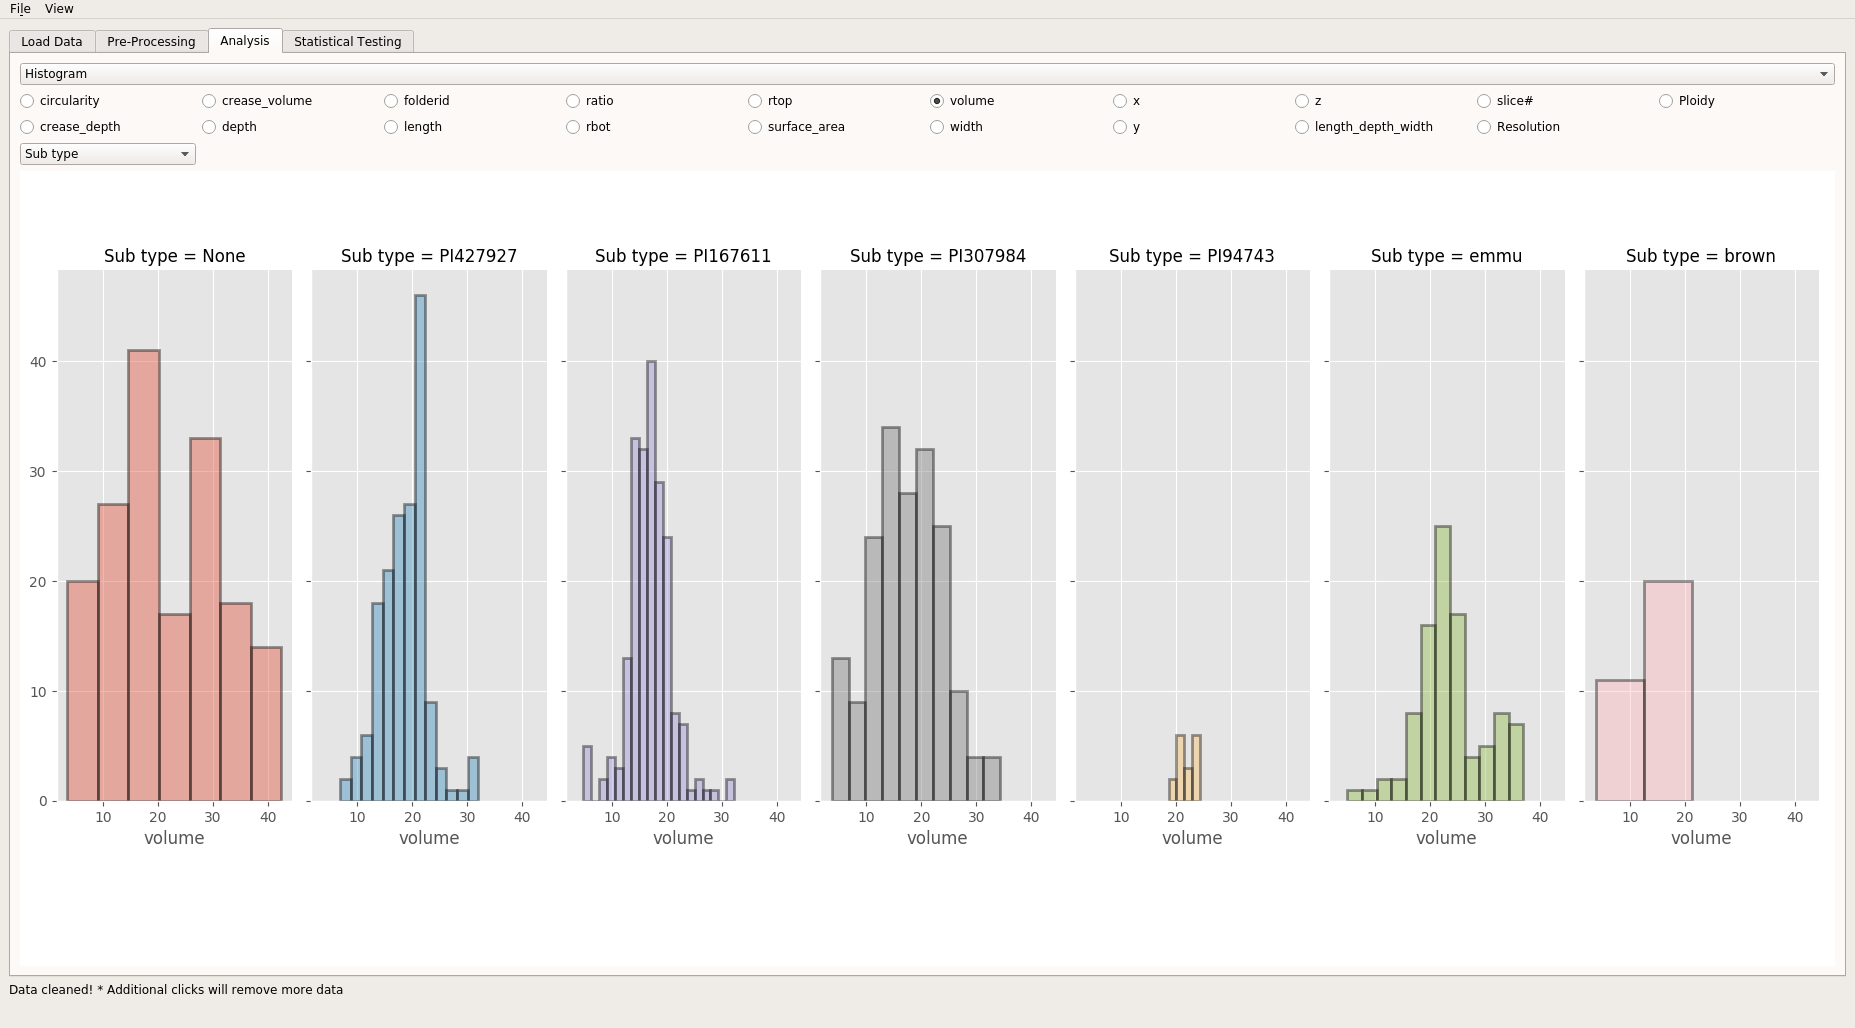
\includegraphics[width=.9\linewidth]{./images/Screenshots/analysis_window_hist_groupby_1_rb_1.png}
\end{center}\\
\hline
\color{ForestGreen}Passed & analysis.py:: hist\_rb\_1 & \begin{center}
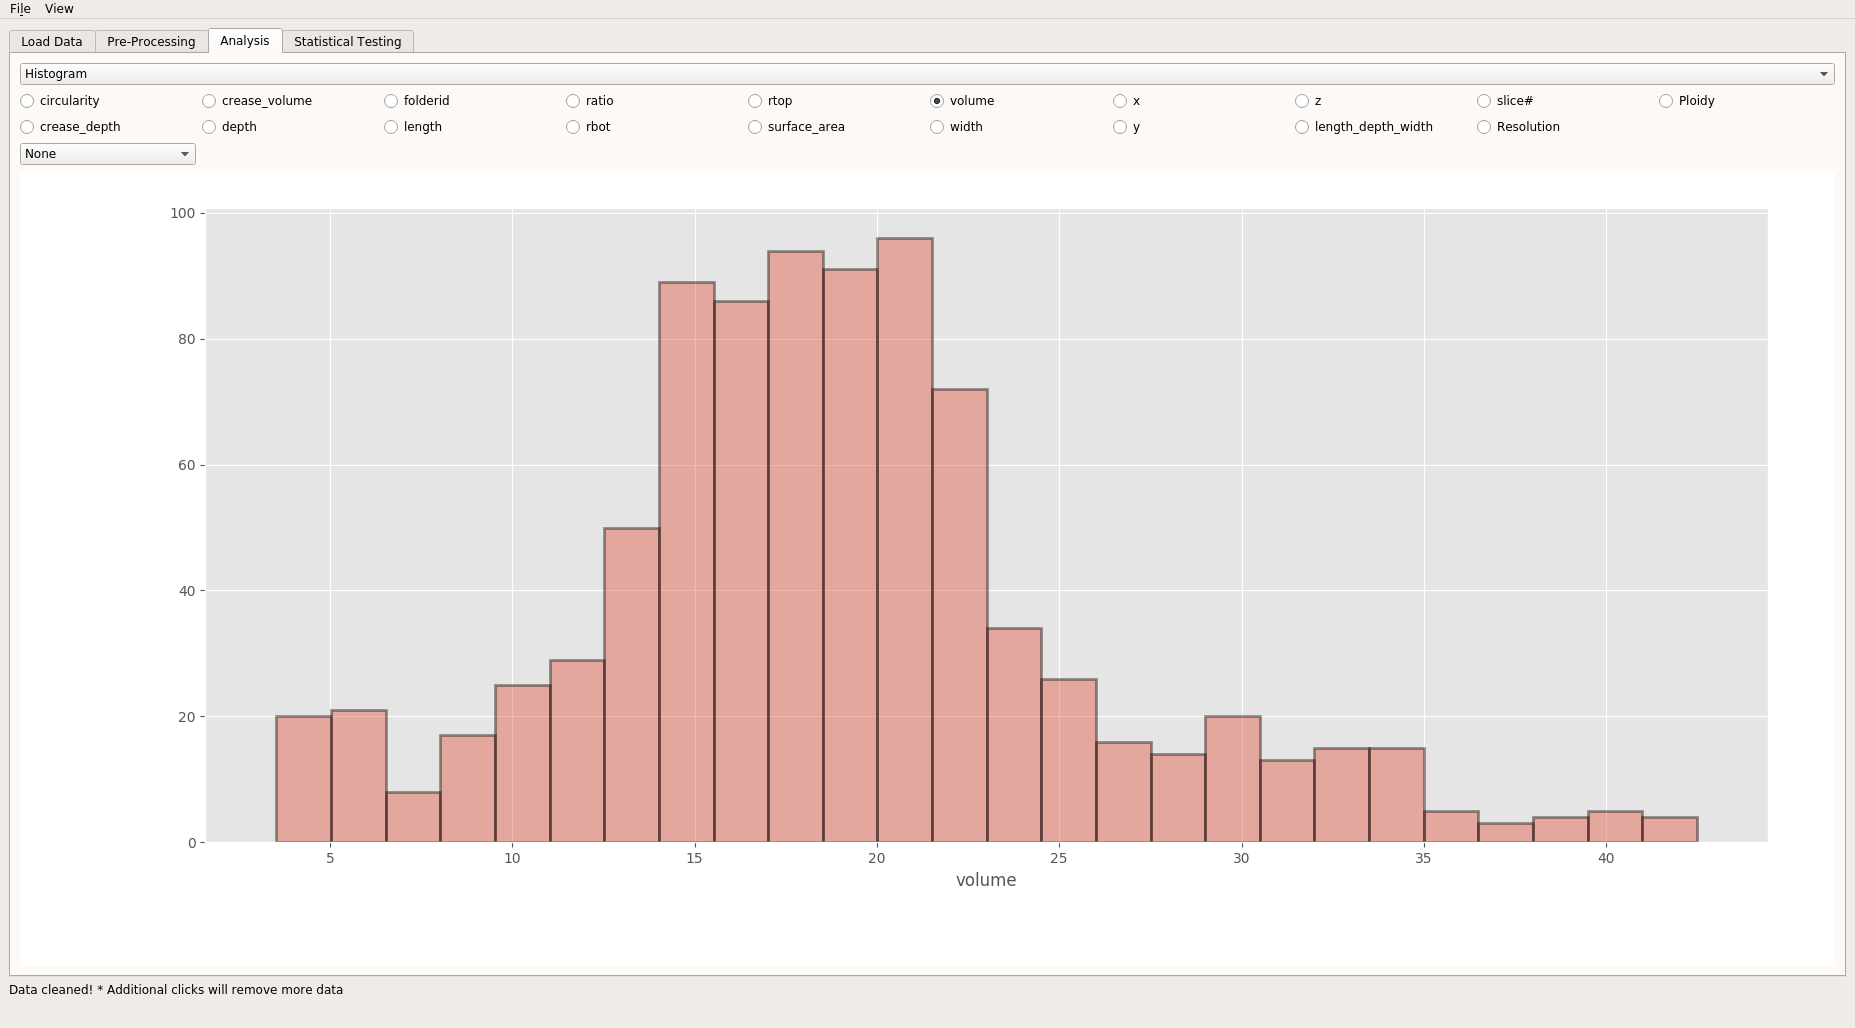
\includegraphics[width=.9\linewidth]{./images/Screenshots/analysis_window_hist_rb_1.png}
\end{center}\\
\hline
\color{ForestGreen}Passed & hypothesis\_tests.py:: bayesg1\_att\_1 & \begin{center}
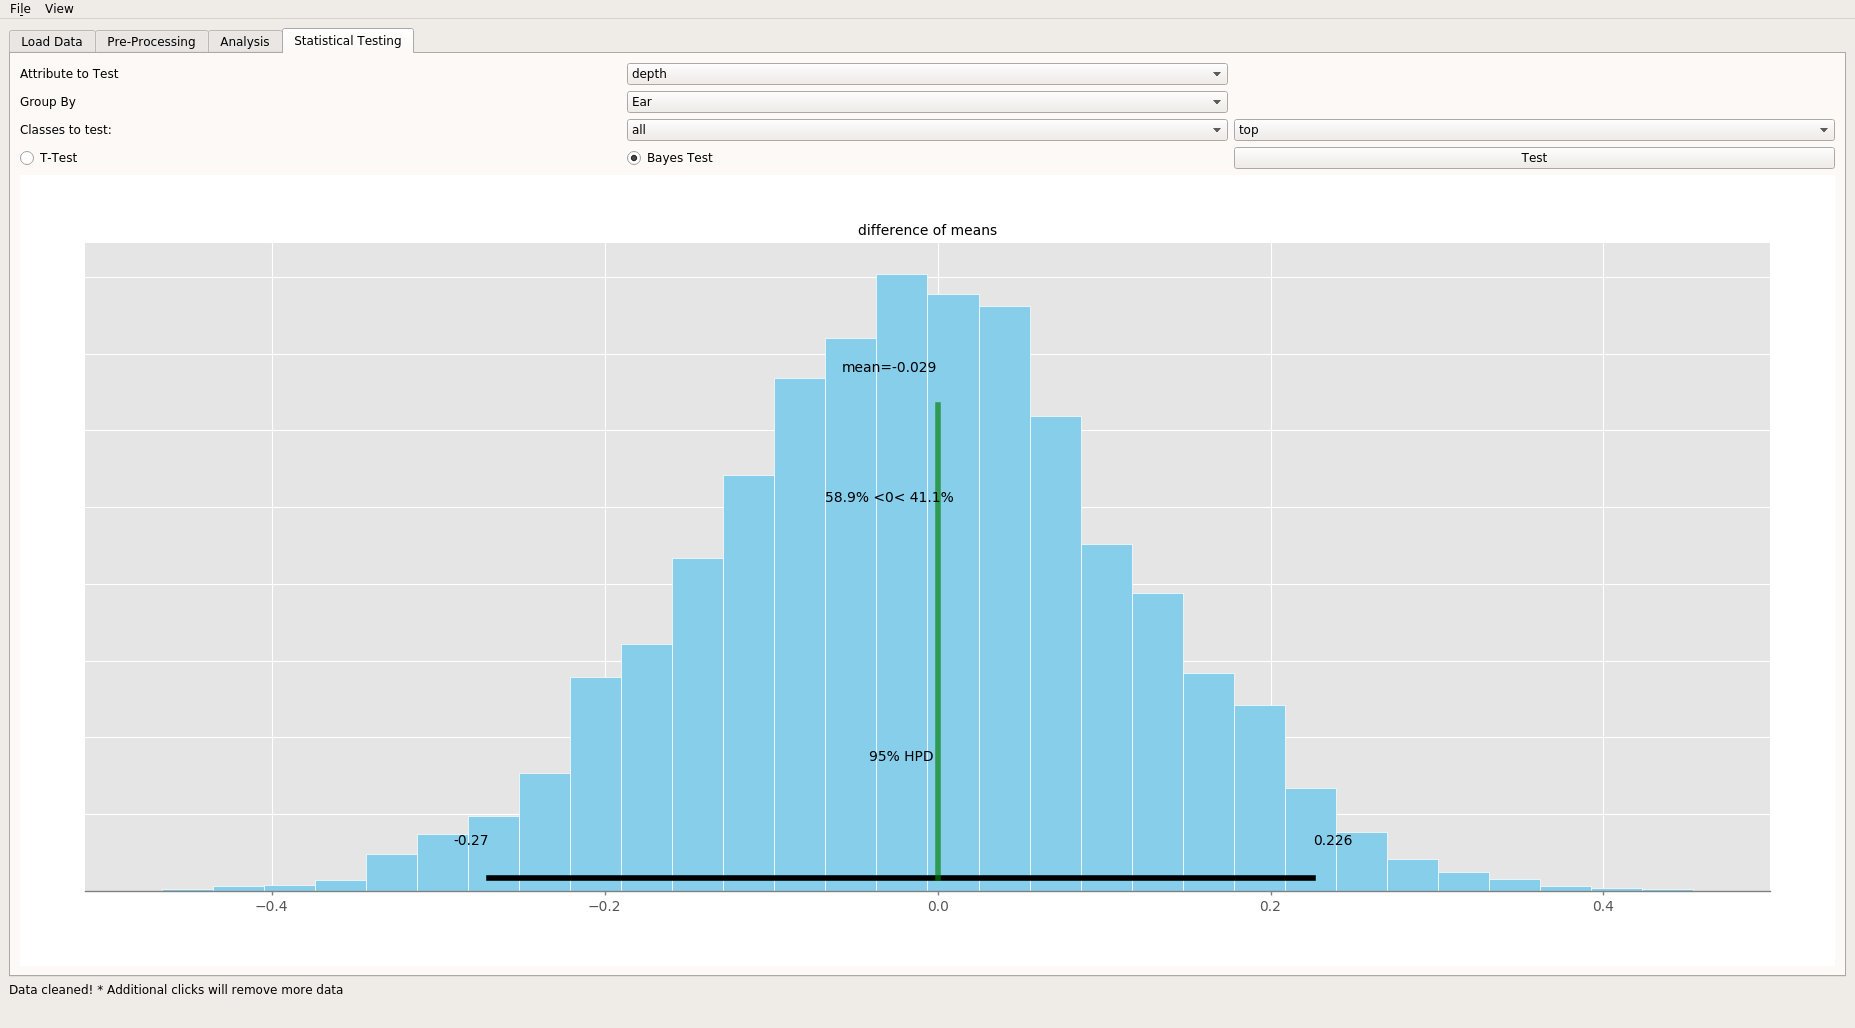
\includegraphics[width=.9\linewidth]{./images/Screenshots/hypothesis_bayestest_g1_att_1.png}
\end{center}\\
\hline
\color{ForestGreen}Passed & hypothesis\_tests.py:: tg1\_att\_1 & \begin{center}
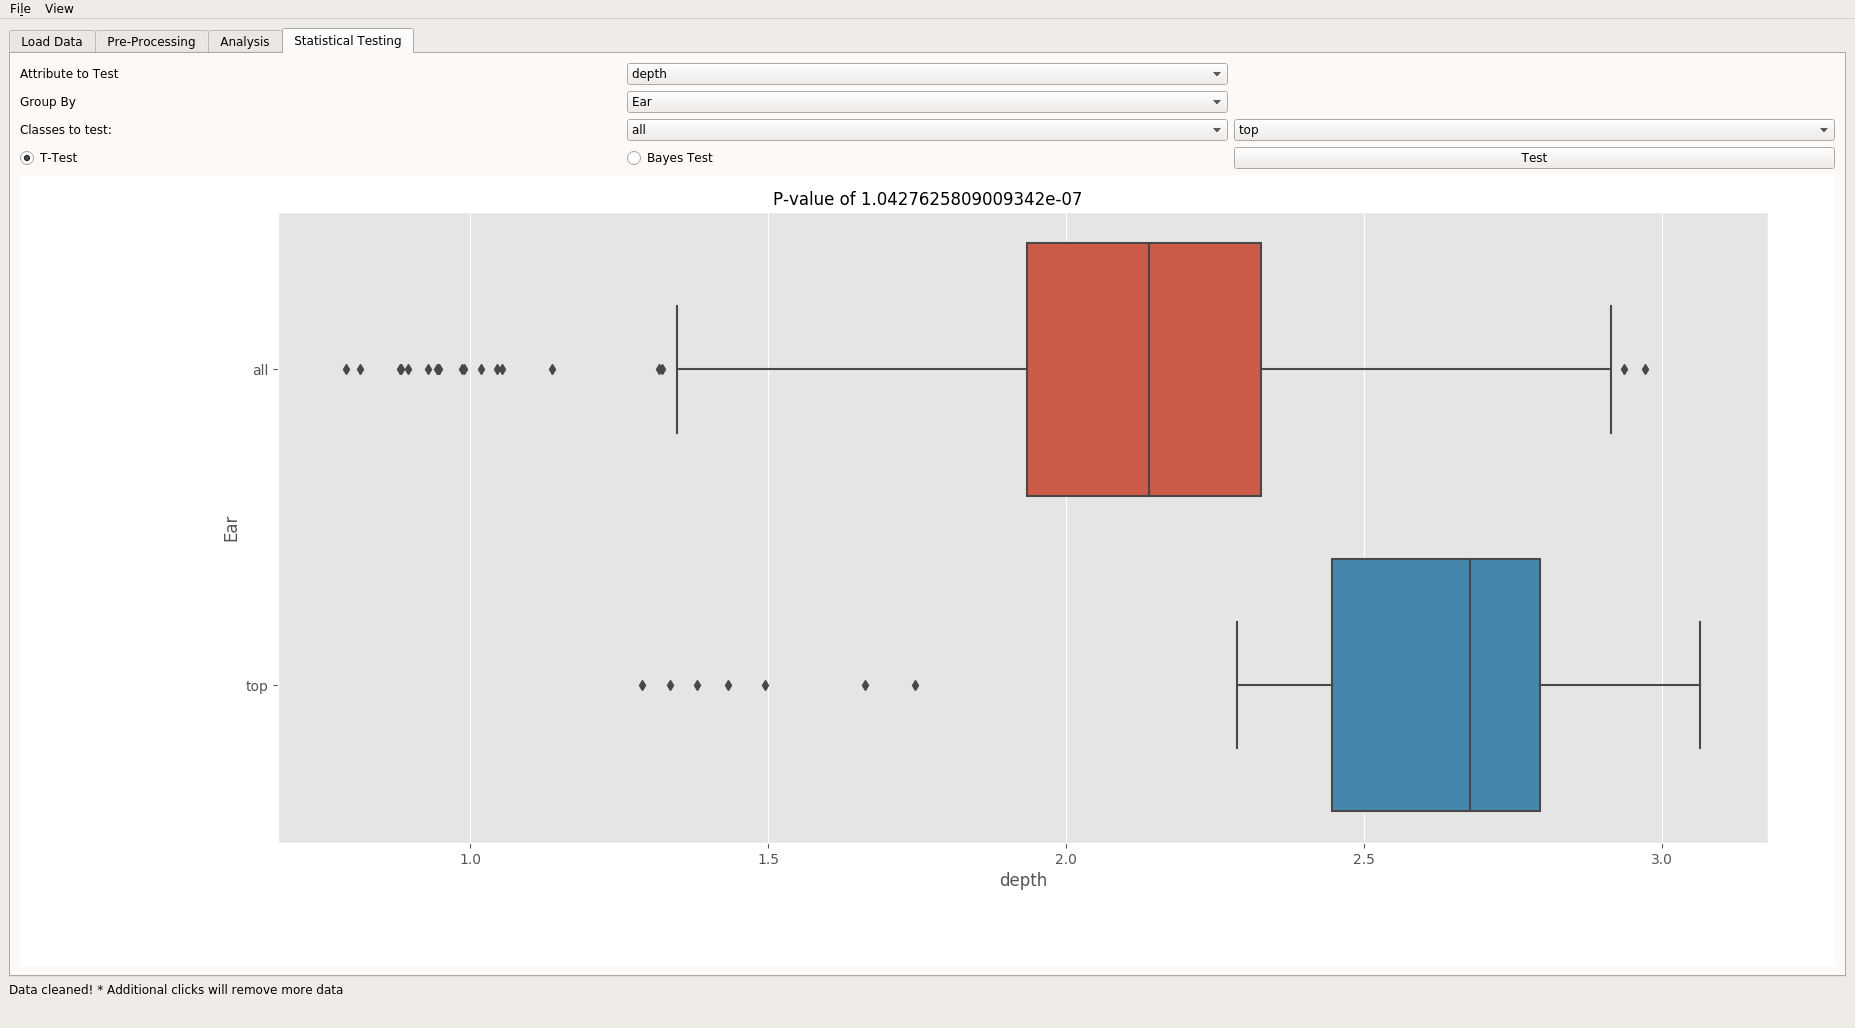
\includegraphics[width=.9\linewidth]{./images/Screenshots/hypothesis_ttest_g1_att_1.png}
\end{center}\\
\hline
\color{ForestGreen}Passed & analysis.py:: box\_rb\_2 & N/A\\
\hline
\color{ForestGreen}Passed & analysis.py:: hist\_groupby\_1\_rb\_2 & N/A\\
\hline
\color{ForestGreen}Passed & analysis.py:: hist\_rb\_2 & N/A\\
\hline
\color{ForestGreen}Passed & analysis.py:: loads & N/A\\
\hline
\color{ForestGreen}Passed & hypothesis\_tests.py:: bayesg1\_att\_2 & N/A\\
\hline
\color{ForestGreen}Passed & hypothesis\_tests.py:: bayesg2\_att\_1 & N/A\\
\hline
\color{ForestGreen}Passed & hypothesis\_tests.py:: bayesg2\_att\_2 & N/A\\
\hline
\color{ForestGreen}Passed & hypothesis\_tests.py:: tg1\_att\_2 & N/A\\
\hline
\color{ForestGreen}Passed & hypothesis\_tests.py:: tg2\_att\_1 & N/A\\
\hline
\color{ForestGreen}Passed & hypothesis\_tests.py:: tg2\_att\_2 & N/A\\
\hline
\color{ForestGreen}Passed & hypothesis\_tests.py:: loads & N/A\\
\hline
\color{ForestGreen}Passed & GUI.py:: startup & N/A\\
\hline
\color{ForestGreen}Passed & load\_data.py:: load\_data\_with\_rachis & N/A\\
\hline
\color{ForestGreen}Passed & load\_data.py:: load\_data\_without\_rachis & N/A\\
\hline
\color{ForestGreen}Passed & preprocessing.py:: clean\_data\_remove\_large & N/A\\
\hline
\color{ForestGreen}Passed & preprocessing.py:: clean\_data\_remove\_none & N/A\\
\hline
\color{ForestGreen}Passed & preprocessing.py:: clean\_data\_remove\_small & N/A\\
\hline
\color{ForestGreen}Passed & preprocessing.py:: clean\_data\_remove \_small\_and\_large & N/A\\
\hline
\color{ForestGreen}Passed & preprocessing.py:: load\_additional\_data & N/A\\
\hline
\color{ForestGreen}Passed & preprocessing.py:: load\_additional\_data \_expected\_fail & N/A\\
\hline
\end{longtable}

\chapter{Methods and Solutions}
\label{sec:org30b71fc}
\section{Data Pipeline}
\label{sec:org8236224}

\begin{figure}[htbp]
\centering
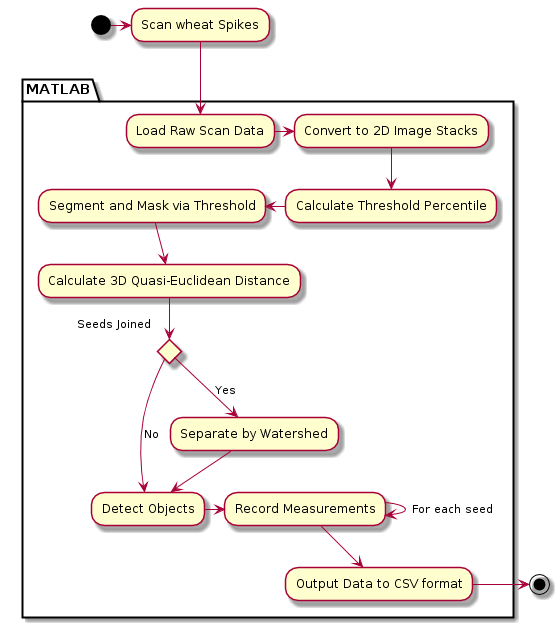
\includegraphics[width=13cm]{./images/matlab.png}
\caption{\label{fig:org5ee2cbc}
Image Processing Pipeline}
\end{figure}

\section{Image Analysis Methods}
\label{sec:orgf123d4e}
\subsection{New Watershed Algorithm}
\label{sec:org94b55fb}

In order to solve the problem of misidentified and joint seeds, from the primitive collection,
a  \emph{quasi-euclidean} distance transform was implemented into the analysis pipeline (figure:). This provided much better results than the previous
\emph{chessboard} transform which had been successful on more uniform data in previous studies \cite{Hughes2017}.

\subsubsection{Quasi-Euclidean algorithm}
\label{sec:org10eec79}

This algorithm measures the total euclidean distance along a set of horizontal, vertical and diagonal
line segments \cite{Pfaltz1966}.

\begin{equation}
\label{eq:org65fa887}
\left | x_1 - x_2 \right | + (\sqrt{2}-1), \left | x_1 - x_2 \right | >\left | y_1 - y_2 \right | (\sqrt{2}-1) \left | x_1 - x_2 \right | ,\textup{otherwise}
\end{equation}



In order to apply this to a 3D space Kleinberg's method is used  \cite{Kleinberg1997}. This allows for nearest neighbour pixels to be sorted by \$k\$-dimensional trees
and enabling fast distance transforms via Rosenfeld and Pfaltz's \emph{quasi-euclidean} method stated in equation:\ref{eq:org65fa887}.
\subsubsection{Effect of Enhanced Watershed algorithm}
\label{sec:org3de4344}
\begin{center}
\begin{figure}[htbp]
\centering
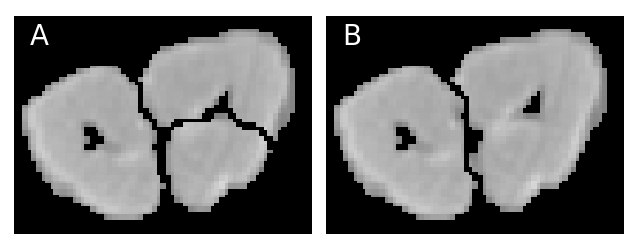
\includegraphics[width=10cm]{./images/chess_quasi.png}
\caption{\label{fig:org20c870f}
\emph{A} showing the chessboard method, \emph{B} improved quasi-euclidean method}
\end{figure}
\end{center}

\subsection{Extracted Grains}
\label{sec:org683ef17}

\begin{figure}[htbp]
\centering
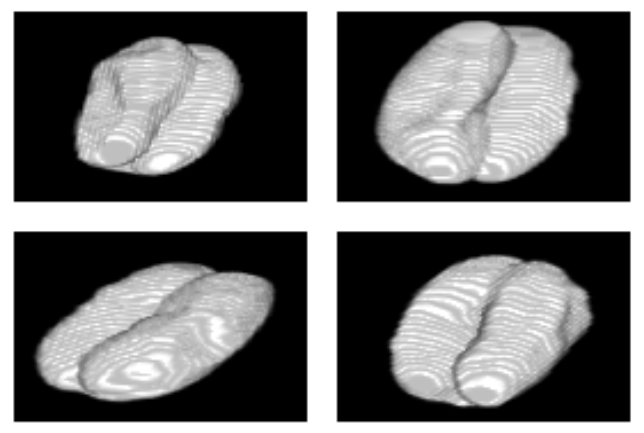
\includegraphics[width=13cm]{./images/ctgrains.png}
\caption{\label{fig:org8b0e2cf}
Individual Wheat grains, rendered in 3D}
\end{figure}

\section{CT Analysing Library Methods}
\label{sec:org6f6a808}
\section{CT GUI Application Methods}
\label{sec:org3252f11}
\section{Data Analysis Methods}
\label{sec:org27c1dcf}

\begin{figure}[htbp]
\centering
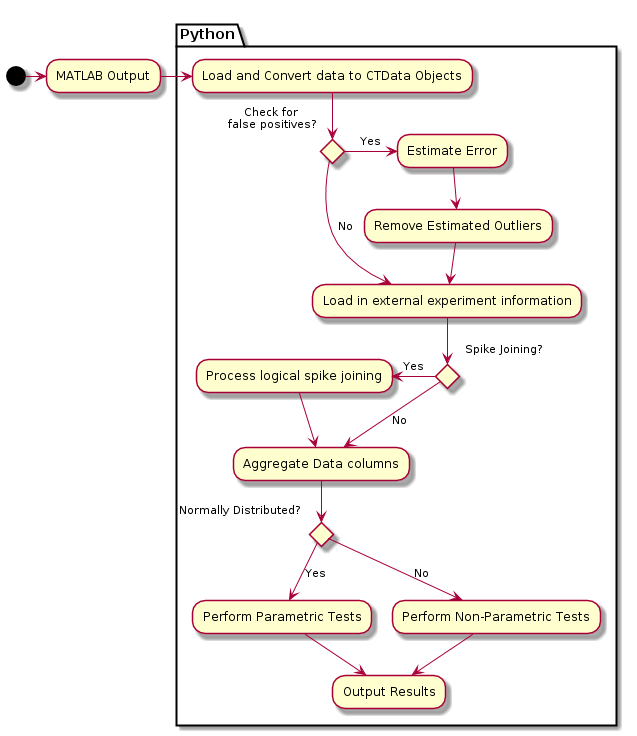
\includegraphics[width=13cm]{./images/pipeline.png}
\caption{\label{fig:org82afe43}
How data is integrated with the CT Analysing Library}
\end{figure}

\chapter{Results}
\label{sec:orgb2e2092}
\chapter{Discussion}
\label{sec:orgbe4077b}
\section{Similar Research}
\label{sec:orgb8e3d7d}
\section{Alternate Solutions}
\label{sec:org99fd3a3}
\chapter{Critical Evaluation}
\label{sec:org5d18240}
\section{Organisational Methods}
\label{sec:org4dff8a7}
\section{Relevance to Degree}
\label{sec:orgaba5251}
\section{Time Management}
\label{sec:orgbb480ba}
\section{Collaborative Work}
\label{sec:org3ce9eb0}
\section{Other Issues}
\label{sec:org0b6e742}
\chapter{Appendix}
\label{sec:orga8c2da1}
\section{\emph{Software Packages Used}}
\label{sec:org808430f}

\subsection{Libraries}
\label{sec:orgcd2859c}
\begin{table}[htbp]
\caption{\label{tab:orgd84b275}
Software libraries used}
\centering
\begin{tabularx}{\textwidth}{|X|X|X|}
\hline
MATLAB Image Processing Toolbox & Numpy & Matplotlib\\
\hline
Seaborn & Scipy & Sklearn\\
\hline
Statsmodels & Pymc3 & Xlrd\\
\hline
PyQt5 & gcc & Pip\\
\hline
\end{tabularx}
\end{table}

\subsection{Tools}
\label{sec:orgb80eece}
\begin{table}[htbp]
\caption{\label{tab:org7ff1320}
Software tools used}
\centering
\begin{tabularx}{\textwidth}{|X|X|X|}
\hline
MATLAB & Python Debugger (PDB) & IPython\\
\hline
Emacs & git & org-mode\\
\hline
Tomviz & ImageJ & \\
\hline
\end{tabularx}
\end{table}

\section{\emph{Glossary}}
\label{sec:org9349aee}
\begin{table}[htbp]
\caption{\label{tab:orgcf3c942}
Dictionary for Terms and acronyms}
\centering
\begin{tabularx}{\textwidth}{|l|X|}
\hline
\textbf{Term} & \textbf{Definition}\\
\hline
\textmu{}-CT & Micro Computed Tomography\\
\hline
Genotype & A genetically distinct individual or group\\
\hline
Phenotype & A physical/measurable trait\\
\hline
Alleles & A variant of a gene\\
\hline
Genus & Classification ranking, below the \emph{family} grouping\\
\hline
Genome & The complete genetic make up of an organism, which defines its individuality\\
\hline
Morphometric & The shape and form of an organism\\
\hline
GUI & Graphical User Interface\\
\hline
PCA & Principal Component Analysis\\
\hline
Spike & A singular stalk of wheat\\
\hline
Spikelet & A group of seeds all forming from the same node in a spike\\
\hline
MVC & Model View Controller - A design pattern for GUIs\\
\hline
OOP & Object Orientated Programming\\
\hline
\end{tabularx}
\end{table}


\section{Wheat Varieties}
\label{sec:org1b143fe}
\begin{table}[htbp]
\caption{\label{tab:orgae2a748}
Dictionary for Wheat names used}
\centering
\begin{tabularx}{\textwidth}{|X|X|}
\hline
\textbf{Used name} & \textbf{Species name}\\
\hline
Monococcum & \emph{Triticum monococcum}\\
\hline
Monococcum Wild & Triticum Boeticum\\
\hline
Tauschii & Aegilops tauschii\\
\hline
Durum & Triticum Durum\\
\hline
Dicoccoides & Triticum Dicoccoides\\
\hline
Dicoccum & Triticum Dicoccum\\
\hline
Ispahanicum & Triticum Ispahanicum\\
\hline
Timopheevii & Triticum Timopheevii\\
\hline
Spelta & Triticum Spelta\\
\hline
Aestivum & Triticum Aestivum\\
\hline
Compactum & Triticum Compactum\\
\hline
\end{tabularx}
\end{table}


\section{\emph{Code Segments and Examples}}
\label{sec:orgdaaa7a3}
\subsection{MATLAB Watershedding}
\label{sec:orgb1af478}

\begin{listing}[htbp]
\begin{minted}[]{octave}
function [W] = watershedSplit3D(A)
  % Takes image stack A and splits it into stack W
  % Convert to BW
  bw = logical(A);
  % Create variable for opening and closing
  se = strel('disk', 5);
  % Minimise object missshapen-ness
  bw = imerode(bw, se);
  bw = imdilate(bw, se);
  % Fill in any left over holes
  bw = imfill(bw,4,'holes');
  % Use chessboard for distance calculation for more refined splitting
  chessboard = -bwdist(~bw, 'quasi-euclidean');
  % Modify the intensity of our bwdist to produce chessboard2
  mask = imextendedmin(chessboard, 2);
  chessboard2 = imimposemin(chessboard, mask);
  % Calculate watershed based on the modified chessboard
  Ld2 = watershed(chessboard2);
  % Take original image and add on the lines calculated for splitting
  W = A;
  W(Ld2 == 0) = 0;
end
\end{minted}
\caption{\label{org6684710}
MATLAB Watershedding function}
\end{listing}

\subsection{Custom Documentation Generator}
\label{sec:org7751265}
\begin{listing}[htbp]
\begin{minted}[]{common-lisp}
(defun populate-org-buffer (buffer filename root)
  (goto-char (point-min))
  (let ((to-insert (concat "* " (replace-regexp-in-string root "" filename) "\n") ))
    (while (re-search-forward
            (rx (group (or "def" "class"))
                space
                (group (+ (not (any "()"))))
                (? "(" (* nonl) "):" (+ "\n") (+ space)
                   (= 3 "\"")
                   (group (+? anything))
                   (= 3 "\"")))
            nil 'noerror)
      (setq to-insert
            (concat
             to-insert
             (if (string= "class" (match-string 1))
                 "** "
               "*** ")
             (match-string 2)
             "\n"
             (and (match-string 3)
                  (concat (match-string 3) "\n")))))helm-semantic-or-imenu
    (with-current-buffer buffer
      (insert to-insert))))

(defun org-documentation-from-dir (&optional dir)
  (interactive)
  (let* ((dir  (or dir (read-directory-name "Choose base directory: ")))
         (files (directory-files-recursively dir "\py$"))
         (doc-buf (get-buffer-create "org-docs")))
    (dolist (file files)
      (with-temp-buffer
        (insert-file-contents file)
        (populate-org-buffer doc-buf file dir)))
    (with-current-buffer doc-buf
      (org-mode))))
\end{minted}
\caption{\label{orgdbf3e7b}
Custom lisp code for generating easy to read documentation}
\end{listing}

\clearpage
\subsection{Self-Documenting Code Example}
\label{sec:org4529e56}
\begin{listing}[htbp]
\begin{minted}[]{python}
def get_spike_info(self, excel_file, join_column='Folder#'):
    """
    This function should do something akin to adding additional
    information to the data frame

    @note there is some confusion in the NPPC about whether to use
    folder name or file name as the unique id when this is made into
    end-user software, a toggle should be added to allow this

    @param excel_file a file to attach and read data from
    @param join_column if the column for joining data is
    different then it should be stated
    """
    try:
        # Grab the linking excel file
        info = pd.read_excel(excel_file,
                             index_col='Folder#')

        features = list(info.columns)
        # Lambda to look up the feature in excel spreadsheet
        def look_up(x, y): return info.loc[x['folderid']][y]

        # Lambda form a series (data row) and apply it to dataframe
        def gather_data(x): return pd.Series(
            [look_up(x, y) for y in features])

        self.df[features] = self.df.apply(gather_data, axis=1)
    except KeyError as e:
        print('Error matching data')
        print(e)
        raise NoDataFoundException
    except AttributeError as e:
        print(e)
        raise NoDataFoundException

\end{minted}
\caption{\label{org9305c03}
Example of code documentation and readability from \emph{data\_transforms.py}}
\end{listing}
\clearpage
\subsection{Setup.py}
\label{sec:orge4211da}
\begin{listing}[htbp]
\begin{minted}[]{python}
from setuptools import setup
setup(name='CT_Analysing_Library',
      version='0.2',
      description='Library used for CT grain analysis at the NPPC',
      url='https://github.com/SirSharpest/CT_Analysing_Library',
      author='Nathan Hughes',
      author_email='nathan1hughes@gmail.com',
      license='MIT',
      packages=['ct_analysing_library'],
      install_requires=['pandas',
                        'numpy',
                        'matplotlib',
                        'seaborn',
                        'scipy',
                        'sklearn',
                        'statsmodels',
                        'pymc3',
                        'xlrd'],
      zip_safe=True)
\end{minted}
\caption{\label{orgd09a84d}
The \emph{setup.py} configuration for the CT Analyser Library}
\end{listing}

\clearpage
\bibliography{library}
\bibliographystyle{IEEEannotU}
\end{document}
